\documentclass[11pt]{article}

\usepackage{pablo}
\usepackage{pgfplots}
\usepackage{numprint}
\usepackage[a5paper,margin=1.8cm]{geometry}

\pagestyle{empty}
\begin{document}

\begin{center}
  {\large
    DM
    ---
    \textsc{Fonctions affines --- Inéquations}
  }
\end{center}

\emph{À rendre le 6 janvier}

\begin{exercice}[Fonctions affines]~
  \begin{enumerate}[(1)]
    \item Calculer l'équation de la droite $\cal D$ passant par les points $A(\frac{1}{3}; 2)$ et $B(1; \frac{2}{3})$.
    \item Dans un repère orthonormé, placer les points $A$, $B$, et tracer la droite $\cal D$. Vérifier la cohérence du tracé.
  \end{enumerate}
\end{exercice}

\begin{exercice}[Problème]~

  \begin{center}
    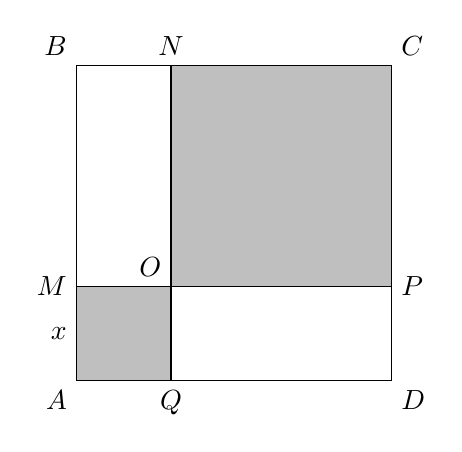
\begin{tikzpicture}[scale=4]
      \draw (0,0) rectangle (1,1);
      \draw [fill=lightgray] (0,0) rectangle (0.3,0.3);
      \draw [fill=lightgray] (1,1) rectangle (0.3,0.3);
      \node[below left] at (0,0) {$A$};
      \node[above left] at (0,1) {$B$};
      \node[above right] at (1,1) {$C$};
      \node[below right] at (1,0) {$D$};
      \node[left] at (0,0.3) {$M$};
      \node[right] at (1,0.3) {$P$};
      \node[above] at (0.3,1) {$N$};
      \node[below] at (0.3,0) {$Q$};
      \node[above left] at (0.3,0.3) {$O$};
      \draw (0,0) -- (0,0.3) node[midway,left]{$x$};
    \end{tikzpicture}
  \end{center}

    $ABCD$ est un carré de côté \numprint[cm]{6} ; $M$ est un point du segment $[AB]$. On pose $x=AM$.

    On construit les carrés $MAQO$ et $ONCP$ tels qu'indiqué sur la figure ci-dessus.

    On appelle ${\cal A}(x)$ l'aire grisée et on cherche à répondre à la question : « Pour quelles valeurs de $x$ la valeur de ${\cal A}(x)$ est-elle supérieure à \numprint[cm\up{2}]{20} ? »

    \begin{enumerate}[(1)]
      \item Quelles sont les valeurs possibles pour $x$ ?
      \item Montrer que ${\cal A}(x)=x^2+(6-x)^2$.
      \item \begin{enumerate}[(a)]
          \item Montrer que le problème revient à résoudre l'inéquation $2x^2-12x+16\geq0$.
          \item Montrer que $2x^2-10x+16=(2x-4)(x-4)$.
          \item Résoudre $(2x-4)(x-4)\geq0$.
          \end{enumerate}
        \item Répondre à la question posée au départ.
    \end{enumerate}
\end{exercice}

\end{document}
